\documentclass{article}

\usepackage{fancyhdr}
\usepackage{enumitem}
\usepackage{amsmath,amsthm,amssymb}
\usepackage{mathtools}
\usepackage{graphicx}
\usepackage[left=0.5in, right=0.5in, top=1in, bottom=1in]{geometry}
\usepackage{bm}
\usepackage[most]{tcolorbox}
\usepackage{tikz}
\usepackage{etoolbox}
\usepackage{microtype}
\usepackage{titlesec}
\usepackage{xcolor}
\usepackage{listings}
\usepackage{indentfirst}
\usepackage{hyperref}
\usepackage{booktabs}
\usepackage{pgfplots}
\usepackage{float}
\tcbuselibrary{listings, breakable}
\usetikzlibrary{positioning, shapes, arrows.meta, decorations.pathreplacing}

\pgfplotsset{compat=1.18}

\setlength{\headheight}{26pt}
\pagestyle{fancyplain}
\setlength{\parindent}{0pt}
\setlength{\parskip}{2ex}
% \addtolength{\topmargin}{10pt}

\lhead{Hossein Bazdar \& AJ Romeo\\ Professor Harry Bendekgey}
\rhead{Tufts, CS135 \\ Page \thepage}


\newcommand{\CustomSubsectiontext}[1]{%
  \vspace{1em}%
  \noindent\textbf{\large #1}\\[0.3ex]%
  \vspace{1em}% very small gap before list or text
}

\newcommand{\CustomSubsectionlist}[1]{%
  \vspace{0.5ex}% small space before heading
  \noindent\textbf{\large #1}\par
  \vspace{0.3ex}% very small gap before list or text
}

\newcommand{\CustomSection}[1]{%
  \vspace{2ex}%
  \noindent\textbf{\LARGE #1}\\
  \vspace{0.5ex}%
  \textcolor{blue!50!cyan}{\rule{0.8\textwidth}{1pt}}\par
}

\tcbset{
  testbox/.style={
    colback=cyan!10,
    colframe=cyan!50,   % border color
    boxrule=0.8mm,      % border thickness
    arc=2mm,
    left=2mm, right=2mm, top=1mm, bottom=1mm
  }
}
\newenvironment{test}[1]{
  \begin{tcolorbox}[testbox]
  \begin{center}
      \large{\texttt{/* #1 */}}
  \end{center}
}{%
  \end{tcolorbox}
}

\tcbset{
  codebox/.style={
    colback=gray!10,    % light gray background
    colframe=gray!50,   % border color
    boxrule=0.3mm,      % border thickness
    arc=2mm,            % rounded corners
    left=2mm, right=2mm, top=1mm, bottom=1mm
  }
}

% Command to display a C function in a gray box
\newcommand{\CFunction}[1]{%
  \begin{tcolorbox}[codebox]
    {#1}
  \end{tcolorbox}
}

\definecolor{codebg}{RGB}{248,248,248}
\definecolor{commentgreen}{RGB}{34,139,34}
\definecolor{keywordblue}{RGB}{0,0,180}
\definecolor{stringred}{RGB}{163,21,21}
\definecolor{framegray}{RGB}{200,200,200}

\newtcblisting{ccode}[1][]{
  listing only,
  listing options={
    language=C,
    basicstyle=\ttfamily\small,
    keywordstyle=\color{keywordblue}\bfseries,
    stringstyle=\color{stringred},
    commentstyle=\color{commentgreen}\ttfamily,
    showstringspaces=false,
    breaklines=true,
    numberstyle=\tiny\color{gray},
    tabsize=4,
    keepspaces=true
  },
  colback=codebg,
  colframe=framegray,
  arc=4pt,
  outer arc=4pt,
  boxrule=0.5pt,
  left=5pt,
  right=5pt,
  top=1pt,
  bottom=5pt,
  breakable,
}

\newtcbox{\Cinline}{on line,
  colback=gray!10,
  colframe=gray!50,
  boxrule=0.3mm,
  arc=1mm,
  left=1mm, right=1mm, top=1mm, bottom=1mm,
  boxsep=0pt,
  fontupper=\ttfamily
}


\titleformat{\subsection}[block]       % 'block' = heading on its own line
  {\large\bfseries}                    % font: large + bold
  {}                                   % no numbering
  {0pt}                                % space between label and title text
  {}                                   % no extra code before text

\titlespacing*{\subsection}
  {0pt}                                % left margin
  {0pt}       % space above
  {0pt}       % space below header before text




\begin{document}
\CustomSection{Problem 1:}
\subsection{Bag-of-Words Design Decision Description}
Our Bag-of-Words design used the sklearn CountVectorizer class rather than implementing our own to determine our vocabulary set. Specifically, we cleaned the data set by converting each word to lowercase, since we decided that there was likely no correlation between case and complexity. Second, we chose to keep stop words like 'the', 'and', and 'is' because we decided that they would help the model differentiate sentences of different structure (a more difficult text may use more stop words to break up complex sentences). Then, we removed occurrences of words in only 1 document or in more than 90\% of documents. This was in part to keep the vocabulary size down (most tests ran around 50k items in vocabulary) and because very rare or very common words have less impact on reading level (super common stop words or made up words likely won't contribute much to a document's rating).  Lastly, we used the ngram parameter from CountVectorizer to account for both single words and bigrams that may give away difficulty such as repetitions of pairs of words like 'not only' or 'such that'. We chose to ignore new words encountered in the test for the same reason we ignored words that appeared in only 1 test document. We used a word count instead of binary values because we believe that the number of time a word is seen in a document is correlated to its complexity.

\subsection{Cross Validation Design Description}
We again used sklearn's StratifiedKFold and GridSearchCV to perform cross validation on our train set. We used 5 folds which landed us with ~4446 in test and ~1111 validation entries per fold. Folds are split at random chosen with shuffled indices in the data set so that there was no bias carried over from the ordering of the train set. We stored the optimal parameters based on each model's performance over AUROC, searching through 7 logarithmically spaced regularization strengths and both L1 and L2 regularization for a total of 14 hyperparameter combinations. AUROC was chosen because it presents a better assessment of classifier performance over other metrics like accuracy. The optimal parameters were assigned to a model using the best\_estimator\_ attribute.

\subsection{Hyperparameter Selection for Logistic Regression Classifier}

\begin{figure}[H]
    \centering
    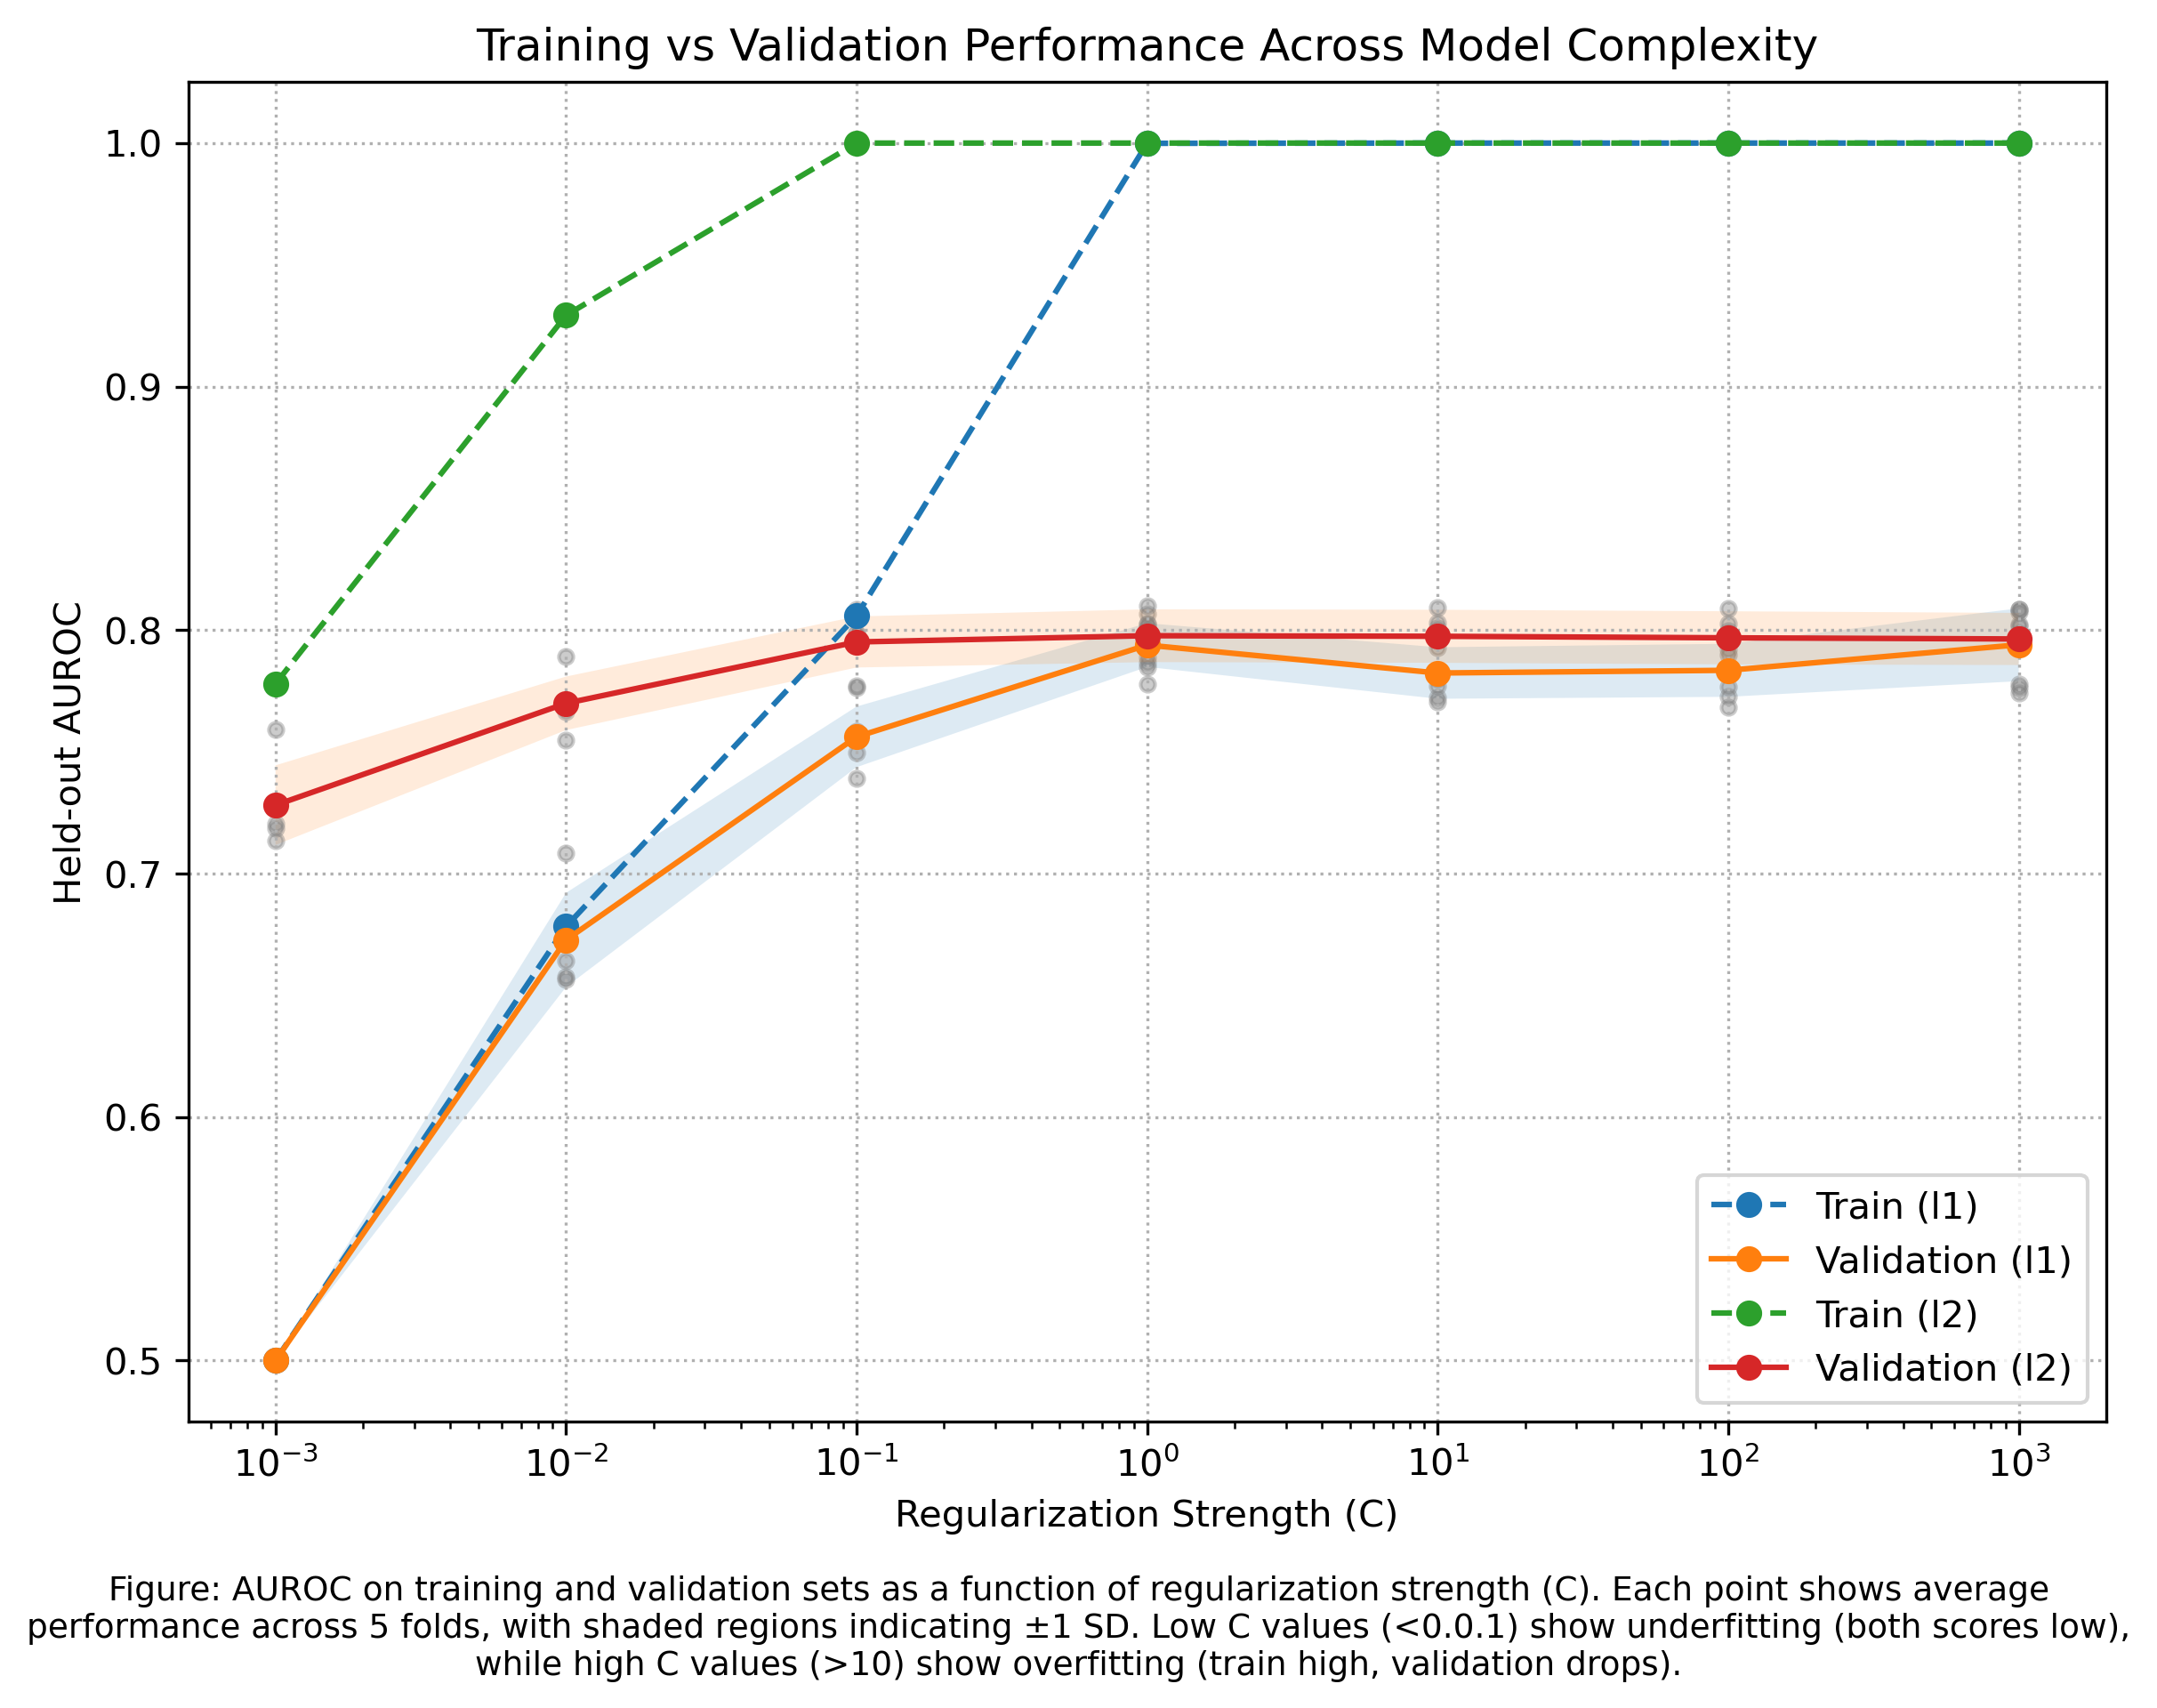
\includegraphics[width=0.55\linewidth]{../p1_hyperparam_train_val_curve.png}
\end{figure}
\newpage
Logistic Regression is a strong choice for determining reading level, as it deals well with sparse features and high dimensions that come with the bag of words data representation. We explored both L1 and L2 regularization as well as 7 regularization strengths spaced over the domain $10^-3$ to $10^3$. The type of regularization affects whether weights will end up as zero (feature gets ignored) or not. We found that L2 performed slightly better, which makes sense, as we wanted words with little weight to still affect the model's prediction and not simply be ignored. For C, a higher value will penalize the weights less than a low value, and it is used to prevent overfitting. The optimal C value fell at 1, where validation AUROC just started to plateau. The model was trained with the liblinear solver from sklearn. No convergence issues were had, as we set the max iterations to 1000. Our final model's parameters were L2 regularization with a C value of 1.0, found via searching over all 14 combinations of C values and both regularization patterns.

\subsection{Analysis of Predictions for the Best Classifier}

\begin{figure}[H]
    \centering
    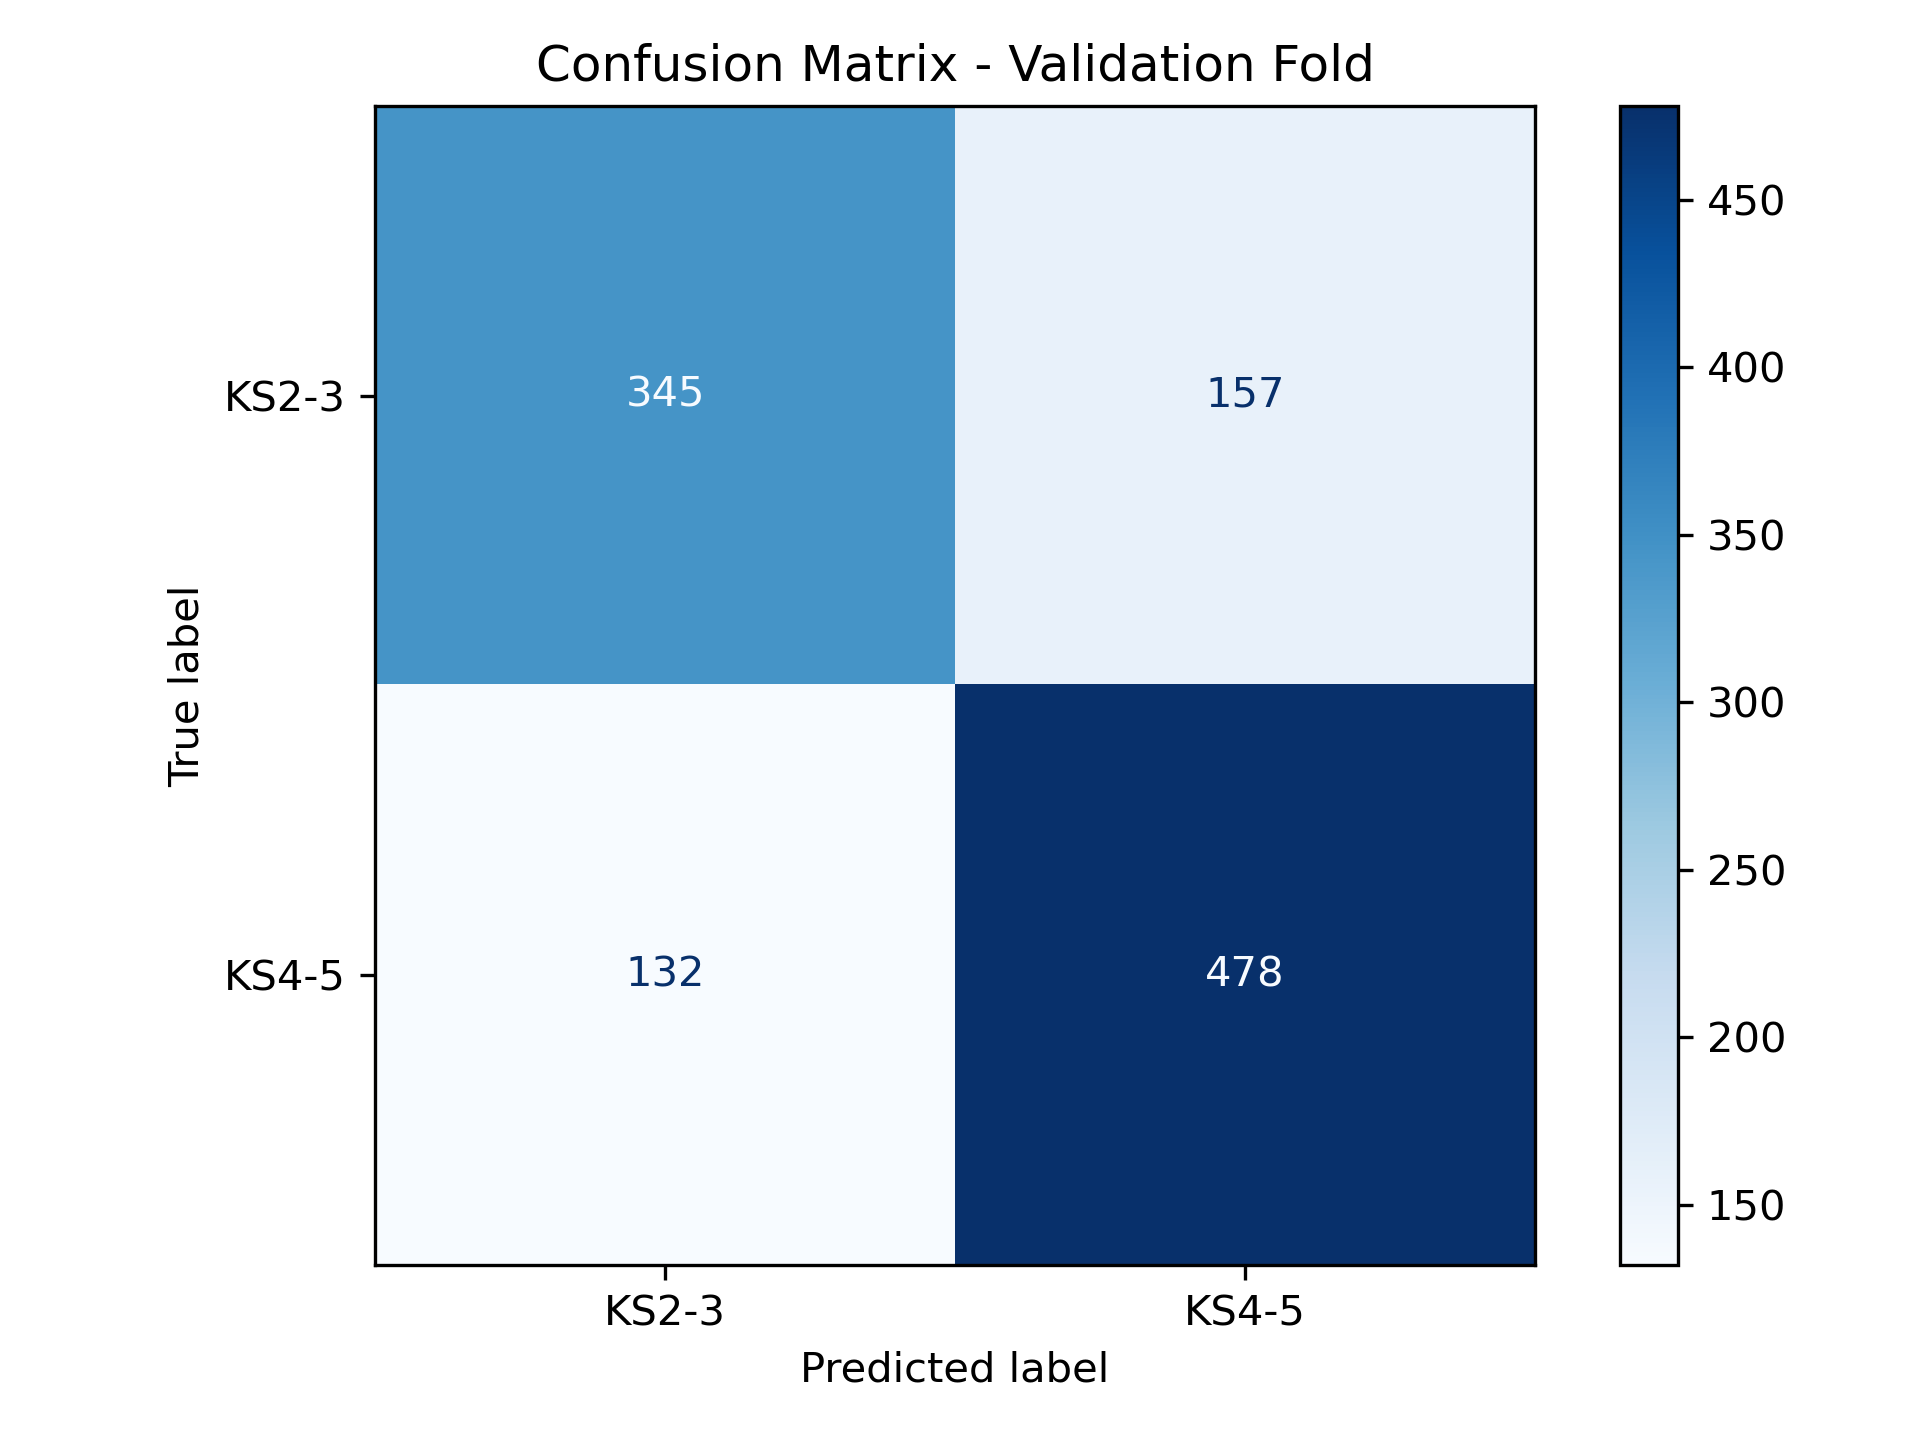
\includegraphics[width=0.55\linewidth]{../p1_confusion_matrix.png}
\end{figure}

Our model tended to over-predict readings as higher level, as shown in the confusion matrix. Looking at the average length of the misclassified texts, they appear to be the same (around 79 words). We did notice, however, that the most misclassified authors wrote lower level texts in much older english, such that the model perceived the old words to mean the text was more difficult than reality. Authors like M. G. Lewis and Robert Louis Stevenson were classified incorrectly often and happened to write around the 18th century. The model tends to perform poorly on documents with a low score but historical language.

\subsection{Report of Performance}


\CustomSection{Problem 2:}
\end{document}

